\label{sec:1}

The DUNE ColdADC is a digitizer ASIC intended for operation in the Deep Underground Neutrino Experiment (DUNE) Far Detectors. It will operated immersed in Liquid Argon (LAr) and will need to operate reliably, without any servicing or component replacement, for over 30 years at a temperature of 88 K.

The ColdADC was implemented in 65 nm CMOS by a team comprised of engineers from Fermilab (FNAL), Brookhaven National Laboratory (BNL), and Lawrence Berkeley National Laboratory (LBNL). The block diagram of the ColdADC is shown in Figure~\ref{fig:coldadc_blockdiagram}.
Each ColdADC has 16 input channels that can either be single-ended or fully differential. The input signals go though a buffer block followed by a Sample-and-Hold (SHA) circuit. The buffer block contains a Single-to-Differential Converter (SDC) and a Differential Buffer (DB). The analog samples after the SHA are multiplexed by a MUX and then digitized by one of two piplined ADCs.
\begin{figure}[h!]
\centering
  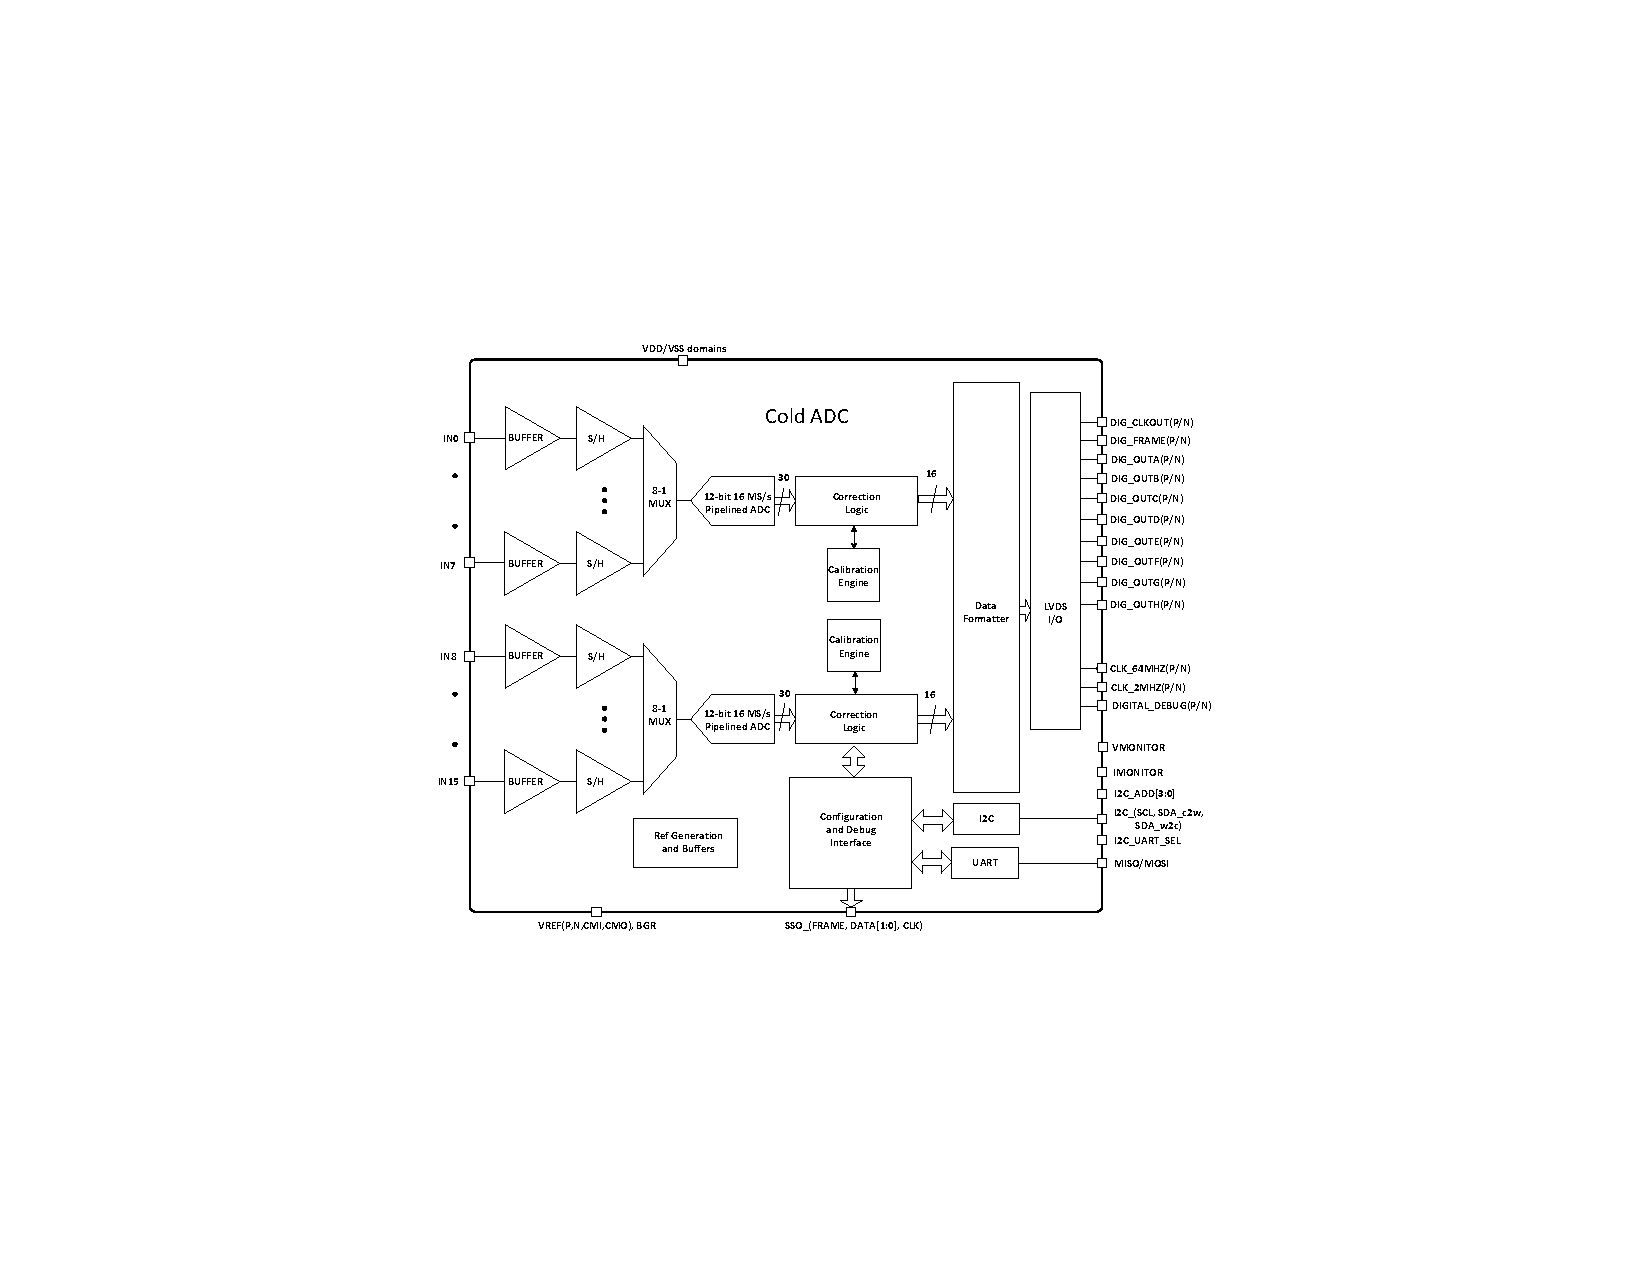
\includegraphics[width=0.8\linewidth]{figures/coldadc_blockdiagram.pdf}
  \caption{ColdADC block diagram.}
  \label{fig:coldadc_blockdiagram}
\end{figure}

In order to mitigate the hot carrier effect (and ensure long operational lifetime at 88 K), the circuits in the ColdADC prototype
%To ensure the ColdADC can operate long-term at 88 K, the ASIC was designed using high-reliability principles developed by BNL. 
%Studies conducted by BNL determined that hot electron effects can cause substrate damage in CMOS circuits and these effects 
%are exacerbated by operation at cold temperature. In order to mitigate hot electrons by reducing the magnitude of the electric 
%field at the gate-drain interface, the circuits on the ColdADC prototype 
are designed with a minimum transistor channel 
length 50\% longer than the minimum length allowed by the process, and the power supplies are kept at 10\% below their nominal 
values. To follow this rule, the synthesized digital circuits use a custom standard cell library with longer 
transistors than the foundry-supplied library. In addition, the architecture of the ADC was chosen as the Pipelined ADC, whose 
performance depends primarily on the matching of ratioed capacitors. Studies conducted by BNL showed capacitor performance 
degraded less than active devices under cold conditions. 

The prototype was submitted for fabrication in late 2018 and received in early 2019. Evaluation is ongoing. 
The first prototype meets essential requirements. The key performance specification, noise, is as expected. Recently the ColdADC has been integrated into a new revision of the DUNE Far Detector Front-End Mother Board (FEMB). Preliminary results are good, and the DUNE Far Detector FEMB is displaying better noise performance than the SBND FEMB, which uses a Commercial Off-the-Shelf (COTS) ADC. This enables the use of a lower gain setting in LArASIC and thus larger dynamic range. The key specifications of the ColdADC compared to the measured results are presented in Table~\ref{tab:coldadc_specs}.
\begin{table}[h]
\centering
\begin{tabular}{|c|c|c|c|}
\hline
\textbf{ Specification } & \textbf{Value} & \textbf{Result} & \textbf{Note}  \\ \hline \hline
Operation Temperature &  Room Temp. (RT) and 88 K & Success & \\ \hline
Sampling Rate & 2 MHz & 2 MHz & \\ \hline
Noise & 200 $\mu$V-rms & 189 $\mu$V-rms & @ LN$_2$ temp \\ 
      &    --            & (302 $\mu$V-rms) & (RT) \\ \hline
Differential Non- & $\pm$0.5 LSB (at 12-bit level) & $+0.2$ to $-0.5$ LSB & @LN$_2$ ; typical values \\
linearity (DNL) & & &  \\ \hline
Integral Non- & $\pm$1 LSB (at 12-bit level) & $+1.2$ to $-1.1$ LSB & @LN$_2$, typical values \\
Linearity (INL) & & &  \\ \hline
Effective-Number- & 11.0 bits & <mean>=10.6 bits & @ LN$_2$ \\ 
of-Bits (ENOB) & & rms=0.3 bits & \\ \hline
No Missing Codes & N/A & Success & @LN$_2$ and RT \\ 
Across Dynamic Range & & & \\ \hline
Crosstalk  & No Specification & $<0.5\%$ & @LN$_2$ \\ 
           &                  & ($<1\%$) &  (RT) \\ \hline
%Power Consumption & $<$50 mW/channel(??) & 24 mW/channel &  \\ \hline
\end{tabular}
\caption{Summary of Results}
\label{tab:coldadc_specs}
\end{table}  

